\documentclass{sigchi}

% Use this section to set the ACM copyright statement (e.g. for
% preprints).  Consult the conference website for the camera-ready
% copyright statement.


%%% Local Variables:
\newcommand{\xray}{XRAY\xspace}
%%% mode: latex
%%% TeX-master: t
%%% End:

% Copyright
\CopyrightYear{2016}
%\setcopyright{acmcopyright}
\setcopyright{acmlicensed}
%\setcopyright{rightsretained}
%\setcopyright{usgov}
%\setcopyright{usgovmixed}
%\setcopyright{cagov}
%\setcopyright{cagovmixed}
% DOI
\doi{http://dx.doi.org/10.475/123_4}
% ISBN
\isbn{123-4567-24-567/08/06}
%Conference
\conferenceinfo{CHI'16,}{May 07--12, 2016, San Jose, CA, USA}
%Price
\acmPrice{\$15.00}

% Use this command to override the default ACM copyright statement
% (e.g. for preprints).  Consult the conference website for the
% camera-ready copyright statement.

%% HOW TO OVERRIDE THE DEFAULT COPYRIGHT STRIP --
%% Please note you need to make sure the copy for your specific
%% license is used here!
% \toappear{
% Permission to make digital or hard copies of all or part of this work
% for personal or classroom use is granted without fee provided that
% copies are not made or distributed for profit or commercial advantage
% and that copies bear this notice and the full citation on the first
% page. Copyrights for components of this work owned by others than ACM
% must be honored. Abstracting with credit is permitted. To copy
% otherwise, or republish, to post on servers or to redistribute to
% lists, requires prior specific permission and/or a fee. Request
% permissions from \href{mailto:Permissions@acm.org}{Permissions@acm.org}. \\
% \emph{CHI '16},  May 07--12, 2016, San Jose, CA, USA \\
% ACM xxx-x-xxxx-xxxx-x/xx/xx\ldots \$15.00 \\
% DOI: \url{http://dx.doi.org/xx.xxxx/xxxxxxx.xxxxxxx}
% }

% Arabic page numbers for submission.  Remove this line to eliminate
% page numbers for the camera ready copy
% \pagenumbering{arabic}

% Load basic packages
\usepackage{balance}       % to better equalize the last page
\usepackage{graphics}      % for EPS, load graphicx instead 
\usepackage[T1]{fontenc}   % for umlauts and other diaeresis
\usepackage{txfonts}
\usepackage{mathptmx}
\usepackage[pdflang={en-US},pdftex]{hyperref}
\usepackage{color}
\usepackage{booktabs}
\usepackage{textcomp}
\usepackage{xspace} % naomi


% Some optional stuff you might like/need.
\usepackage{microtype}        % Improved Tracking and Kerning
% \usepackage[all]{hypcap}    % Fixes bug in hyperref caption linking
\usepackage{ccicons}          % Cite your images correctly!
% \usepackage[utf8]{inputenc} % for a UTF8 editor only

% If you want to use todo notes, marginpars etc. during creation of
% your draft document, you have to enable the "chi_draft" option for
% the document class. To do this, change the very first line to:
% "\documentclass[chi_draft]{sigchi}". You can then place todo notes
% by using the "\todo{...}"  command. Make sure to disable the draft
% option again before submitting your final document.
\usepackage{todonotes} % naomi
\usepackage[normalem]{ulem} % also naomi

% Paper metadata (use plain text, for PDF inclusion and later
% re-using, if desired).  Use \emtpyauthor when submitting for review
% so you remain anonymous.

\def\plaintitle{XRAY: Inspector Tools For Designers}
\def\plainauthor{First Author, Second Author, Third Author,
  Fourth Author, Fifth Author, Sixth Author}
\def\emptyauthor{}
\def\plainkeywords{Web design; design systems; inspector tools; experimentation; human factors; developers; designers. 
}
\def\plaingeneralterms{Documentation, Standardization}

% llt: Define a global style for URLs, rather that the default one
\makeatletter
\def\url@leostyle{%
  \@ifundefined{selectfont}{
    \def\UrlFont{\sf}
  }{
    \def\UrlFont{\small\bf\ttfamily}
  }}
\makeatother
\urlstyle{leo}

% To make various LaTeX processors do the right thing with page size.
\def\pprw{8.5in}
\def\pprh{11in}
\special{papersize=\pprw,\pprh}
\setlength{\paperwidth}{\pprw}
\setlength{\paperheight}{\pprh}
\setlength{\pdfpagewidth}{\pprw}
\setlength{\pdfpageheight}{\pprh}

% Make sure hyperref comes last of your loaded packages, to give it a
% fighting chance of not being over-written, since its job is to
% redefine many LaTeX commands.
\definecolor{linkColor}{RGB}{6,125,233}
\hypersetup{%
  pdftitle={\plaintitle},
% Use \plainauthor for final version.
%  pdfauthor={\plainauthor},
  pdfauthor={\emptyauthor},
  pdfkeywords={\plainkeywords},
  pdfdisplaydoctitle=true, % For Accessibility
  bookmarksnumbered,
  pdfstartview={FitH},
  colorlinks,
  citecolor=black,
  filecolor=black,
  linkcolor=black,
  urlcolor=linkColor,
  breaklinks=true,
  hypertexnames=false
}

% create a shortcut to typeset table headings
% \newcommand\tabhead[1]{\small\textbf{#1}}

% End of preamble. Here it comes the document.
\begin{document}

\title{\plaintitle}

\numberofauthors{3}
\author{%
  \alignauthor{Leave Authors Anonymous\\
    \affaddr{for Submission}\\
    \affaddr{City, Country}\\
    \email{e-mail address}}\\
  \alignauthor{Leave Authors Anonymous\\
    \affaddr{for Submission}\\
    \affaddr{City, Country}\\
    \email{e-mail address}}\\
  \alignauthor{Leave Authors Anonymous\\
    \affaddr{for Submission}\\
    \affaddr{City, Country}\\
    \email{e-mail address}}\\
}

\maketitle

\begin{abstract}
Numerous tools have been created to facilitate developers' borrowing of code from live websites and design examples. However, little work has been done to improve the experience of designers working on partially-developed or live sites. This paper introduces \xray, inspector tools for designers (Figure~\ref{fig:xray_screenshot}). Unlike traditional inspector tools, \xray allows the designer to adjust fonts, colors, margins, and padding within the browser without ever needing to look at HTML or CSS, making this technical, traditionally code-based task more approachable for designers. \xray promotes the use of design systems by only suggesting styling options that exist in the current design system and highlighting where current aesthetics violate the design system. \xray also improves designer-developer communication by allowing people in different locations are able to make live edits to a website collaboratively. \xray allows users to export a document with all changes at the end of their session. 
Moreover, a 12 person user study with novices and a 12-person user study with professional designers showed that people were xx\% more efficient, yy\% more successful, and experimented more by using zz\% more styles when they used \xray, than when they used the standard industry tools. 
\end{abstract}


% Running questions/comments: 
% are we calling users: users? people? designers? 
% I know every other sentence starts with the word "XRAY" and I will eventually get around to fixing it

\category{H.5.m.}{Information Interfaces and Presentation
  (e.g. HCI)}{Miscellaneous} \category{See
  \url{http://acm.org/about/class/1998/} for the full list of ACM
  classifiers. This section is required.}{}{}

\keywords{\plainkeywords}
\section{Introduction}


\begin{figure}
    \centering
    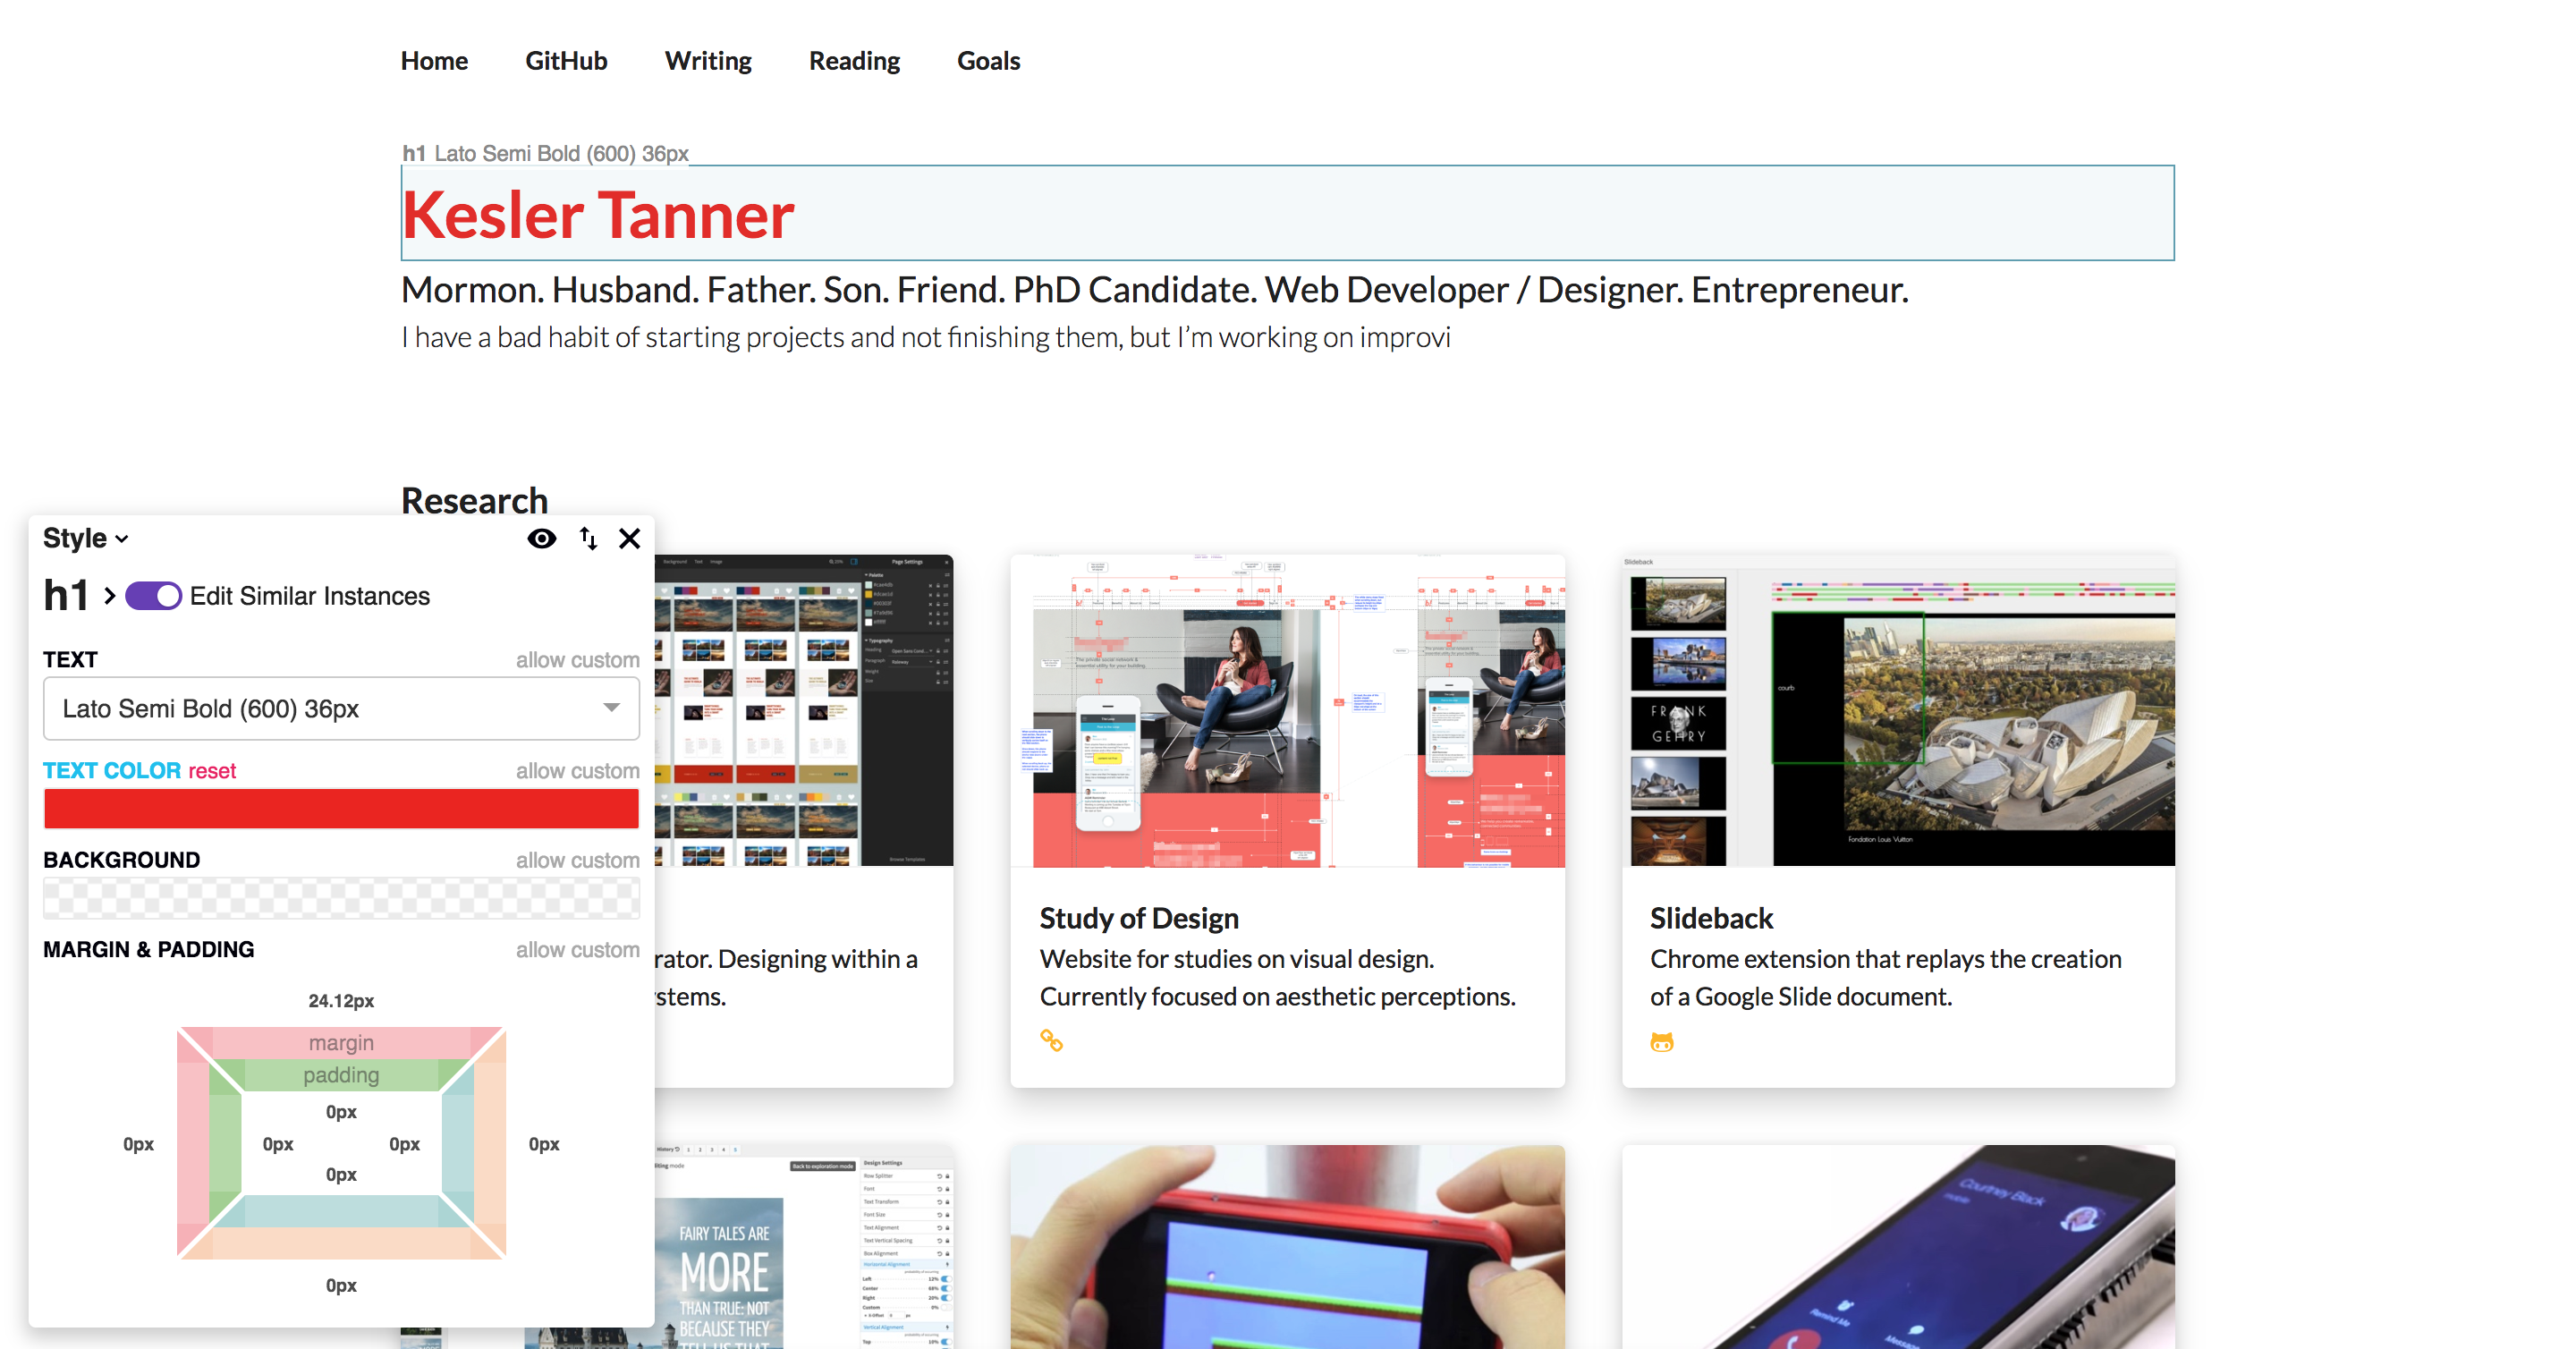
\includegraphics[width=\columnwidth]{figures/image.png}
    \caption{A screenshot of the \xray user interface and the menu for [fonts? colors? margin/padding?]}  
    \label{fig:xray_screenshot}
\end{figure}

By definition, designers plan the UI of software and developers write the code. Although some designers can code and some developers are artistically savvy, most professionals in industry specialize. Creating a finished projected is a collaborative and iterative process. For example, if a company was preparing to launch a new website, the designer would create a mockup of how the product should look and send it to the developer. The developer would code it, and send it back to the designer. No first draft is flawless; the designer would next communicate the mistakes to the developer. 

Some designers will meet with the developers, sitting next to them and explaining what needs to be changed. However, that is very time-consuming for both the developer and designer. Other designers might send an email with a checklist of what needs to be fixed, but matching the block of test to the website gets confusing very quickly. In reality, it is most common for the developer to ``redline'' by marking up a screenshot of the website using tools like Sketch or InVision, such as in Figure~\ref{fig:markup_redline_website} as taken from Moore's 2017 Medium article \cite{digital_whiteboards_moore_medium_2017}. 


The ability to write comments on a screen simplifies the revision process. Instead of writing an essay for each bullet point (``the icon of a drill on the top left of the home page should be enclosed by a circle instead of a square''), the designer can draw an arrow to the icon they are dissatisfied with and write ``should be a circle.'' 

However, when it comes to colors, padding, and other sizing issues, detail is key. Instead of saying ``this black should match the black background on the homescreen'', why not just tell the developer the hexcode should be \#000000? Additionally, prior work shows the benefits of experimentation, yet writing notes on screenshots does not really provide the opportunity to expirement and try new ideas. Ideally, when the designer notices that the line height is too large, they would have the opportunity to see what the page would look like with 1.1em, 1.2em, and 1.3em before telling the developer which one is best. 

\begin{figure}
    \centering
    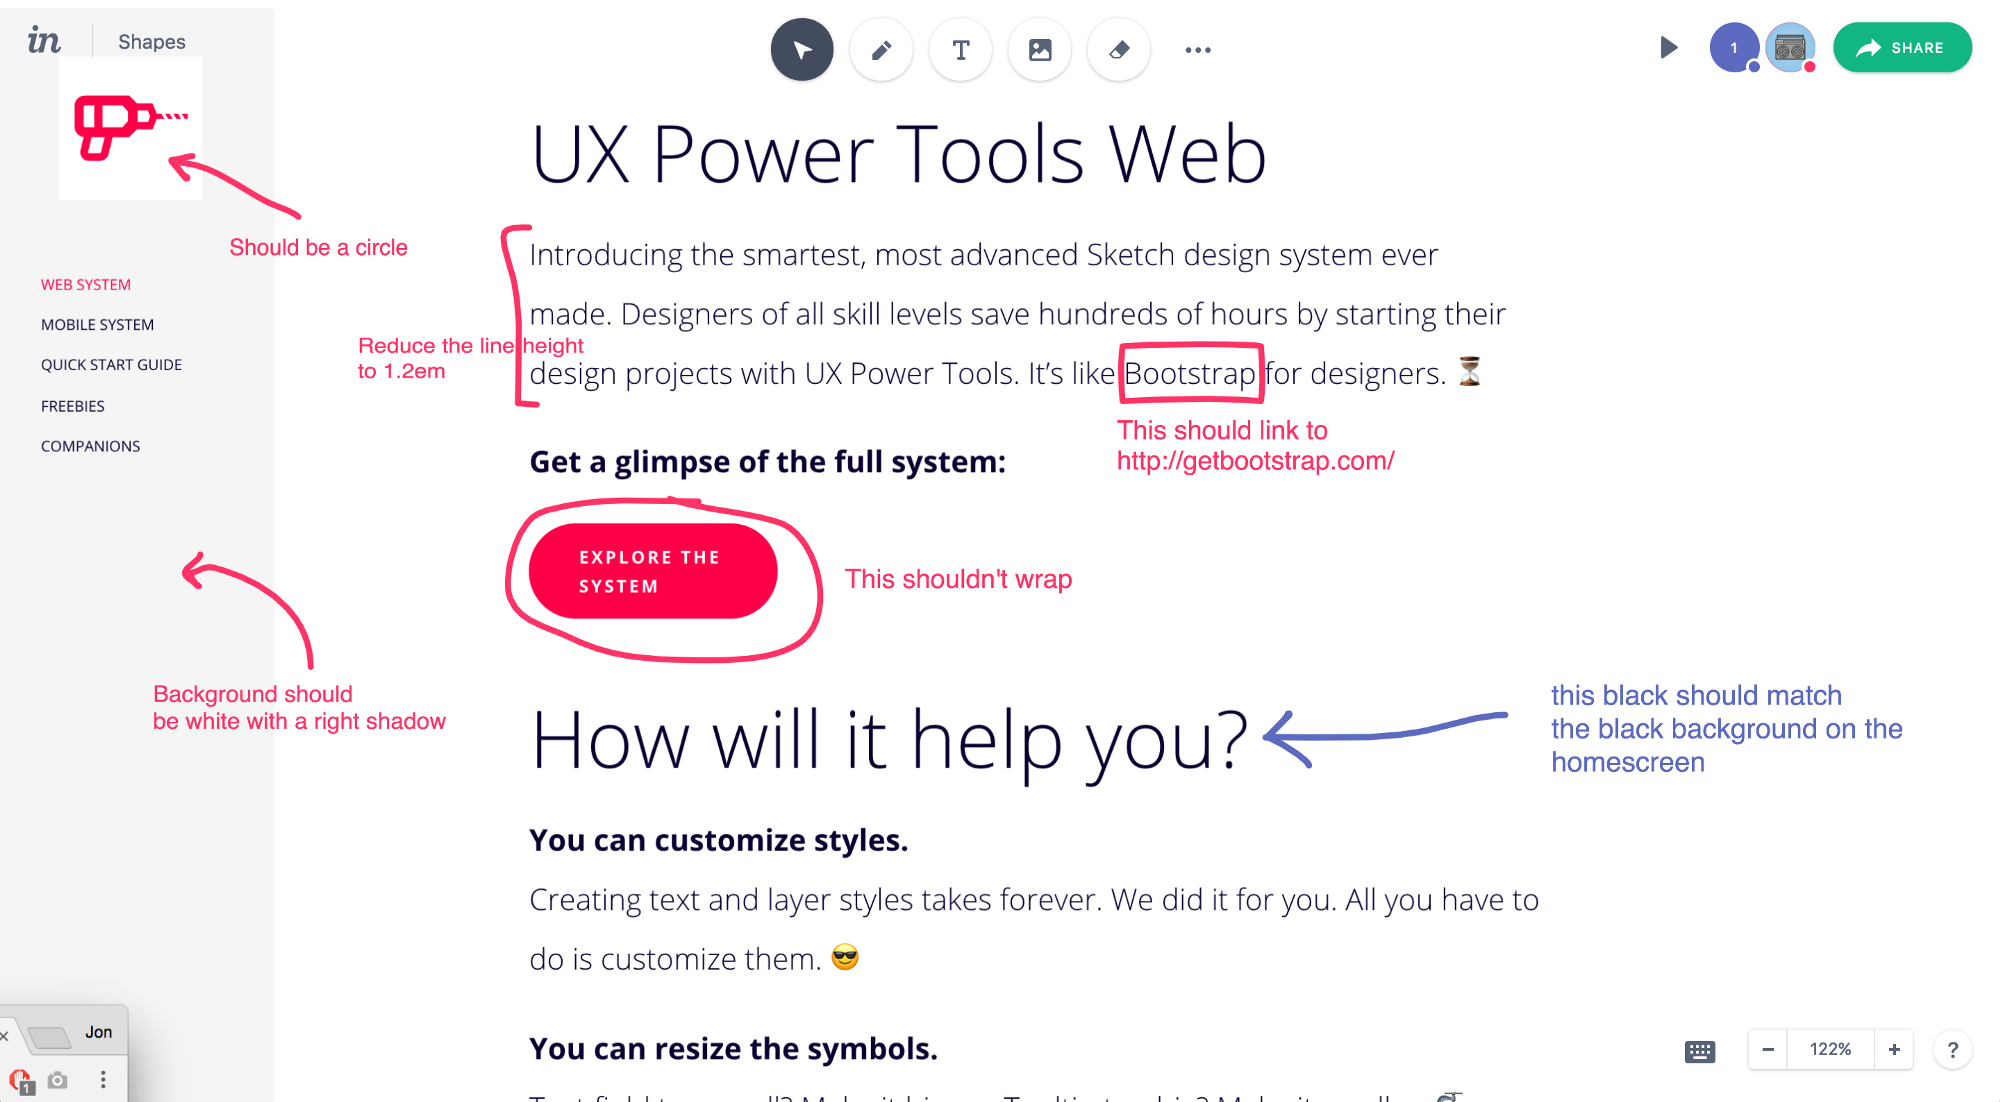
\includegraphics[width=\columnwidth]{figures/screenshot_redline_found_google.png}
    \caption{Example of a ``redline'' or markup of website that a designer might send to a developer}
    % https://medium.com/ux-power-tools/invision-freehand-digital-whiteboarding-bf83639c1184
    % \cite{digital_whiteboards_moore_medium_2017
    \label{fig:markup_redline_website}
\end{figure}


% of colors, fonts, spacing rules, and a library of pre-built widgets used in one website, app, or company.  
Currently, the developers are gatekeepers: they control the design and aesthetics of a finished product even though they do not have the knowledge or training that a designer does. The designers are in the uncomfortable position of knowing exactly how the final product should look, but are unable to create it themselves. 

In order to provide designers with more control, many companies are creating design systems. Just as developers use a style guide in order to have a standardized way of writing code, designers create design systems to standardize the look and feel of a product. 
% Many customers associate certain fonts or color palettes with a particular company logo. 

Most companies strive to be consistent in their use of colors and fonts across websites, emails, advertising campaign, and apps [cite]. Design systems evolved from these style guides. Couldwell walks through how WeWork created a design system which contains not only font families, font sizes, and colors, but also templates, patterns (which include recurring elements or practices like navigation, cards, tables, or alerts), and components (pre-built widgets, such as buttons, sliders, or inputs, selects, toggles, avatars, tooltips, and etc) \cite{design_system_at_plasma_couldwell_medium_2017}. 

% there aren't research papers about design systems (site that airbnb paper, large companies that have these design systems) 

% (we need this common vocabulary/language/common ground to facilitate designer/developer communication. Take what exists in the code and get it into figma/other graphic editor environments. \#unification) 

% Both programmers and web designers look at websites for design inspiration and at snippets of code for guidance. Researchers and industry professionals have made developers tools to enable these programmers and designers to learn more from these examples. However, many of these tools are geared towards those who are comfortable with code. 

When developers and designers face seemingly small questions like ``How should we format the time/date/currency?'' or ``What kind of color/typeface/button should I use?'' or ``Should this be sentence case or title case?'', the design system can evolve to hold these answers \cite{what_is_design_system_couldwell_medium_2017}. Often a [file type] or [photoshop file], the design system can contain images of what these fonts, colors, and widgets look like, as well as the code to make them. This prevents developers from making the same buttons over and over for each website, and ensures that the color, shadow, and animated reaction for each click or hover over the button will be exactly the same \cite{what_is_design_system_couldwell_medium_2017}. 

Although the use of design systems is spreading rapidly in industry, we are not aware of any research regarding the creation or use of them. Companies including [list them] are currently using them; some began creating their design system as early as [year]. 

In order to 1. improve the experience of web designers, 2. improve their collaboration with developers, and 3. to promote the use of design systems, we built \xray (Figure~\ref{fig:xray_screenshot}), design-oriented inspector tools for developers. Unlike traditional inspector tools, \xray allows the designer to adjust fonts, colors, margins, and padding without ever needing to look at HTML or CSS, making this technical, traditionally code-based task more approachable for designers. 

% ALSO, (A. Allows designer to work in same medium as developers (as opposed to graphical tools like sketch), and B. Allows designer to better understand how websites are made/visualize element style and positioning i. Margin v. padding, etc)

\xray makes the following contributions: 

\begin{itemize}
    \item A novel set of inspector tools, designed for those who do not need to understand how HTML and CSS work. \xray allows users to adjust fonts, colors, margins, and padding on live sites without ever looking at any code. 
    
    \item \xray focuses on design systems. By only suggesting choices that are in the current design system, it helps novice designers be consistent. \xray provides the option to override these design guidelines, allowing users to expand the design system by adding new rules. When users redefine an aspect of their design system, \xray automates consistency, letting the changes percolate through not only the current page but the entire website, persisting even after page reloads. \xray highlights where a site breaks from the design systems, letting users quickly identify possible issues. 
    
    \item Designer-developer communication is improved because people in different locations are able to make live edits to a website collaboratively. At the end of a session, designers can export a document with all of their final changes noted in HTML and CSS to give to the developer.  
    
    \item A within-subject evaluation of \xray in comparison to the industry standard of using Sketch(c) to note flaws in a website. We had a total of 24 partcipants, half of whom were design professionals with a minimum of five years' experience, and half of whom were design students at a competetive private university. Our results showed that people were xx\% more efficient, yy\% more successful, and experimented more by using zz\% more styles when they used \xray, than when they used the standard industry tools.
\end{itemize}


\section{Related Works}
Currently, in industry, the best way for designers to give feedback to developers is through marked up screenshots created in Sketch. The purpose of \xray is to allow designers more control over the design of a website. In essence, \xray is a designer's version of the developer tools that exist in most browsers. First, we discuss research and tools that were created to assist design. Second, we discuss research and tools for development. Third, we discuss why \xray is needed to help bridge the divide between developers and designers.  

\subsection{Designers}
Examples play a critical role in the creative process \cite{getting_inspired_designs_in_creativity_Herring_CHI_2009}. Research has discussed the role of examples in non-routine design \cite{creativity_in_design_activities_Bonnardel_CandC_1999}, how different examples are used in design \cite{getting_inspired_designs_in_creativity_Herring_CHI_2009}, and the impact of examples \cite{effects_of_examples_on_design_activities_Purcell_1992_kbc}. Researchers have created galleries of designs in order to provide designers with examples.

Because web search has historically been done with keywords \cite{cueflik_interactive_concept_leraning_Fogarty_CHI_2008}, looking for examples with specific characteristics can be difficult. The 1997 Design Galleries presented users with a variety of options to assist in parameter setting for animation, image rendering, or volume rendering \cite{designGalleries_mitsubishi_Marks_SIGGRAPH_1997}. More recent work has included curated databases of web designs, allowing users to search for examples with similar qualities or look for examples that vary on a particular axis \cite{interactive_example_galleries_Lee_CHI_2010}, search for examples with stylistic keywords \cite{dtour_Ritchie_UIST_2011} or via the input of a rough sketch \cite{retrieving_websites_with_sketches_example_based_design_hashimoto_igarashi_EUROGRAPHICS_EWSBIM_2005}. 

The inherent drawback to human-curated databases is the time required to create and maintain them. Data mining websites, apps and other software for design or other information is discussed in the related works of this thesis \cite{mining_data_phd_thesis_uc_boulder_alharbi_yeh_2016}. Work has included platforms to collect and annotate web designs on small-scale of 300 web pages \cite{learning_on_web_design_Satyanarayan_CHI_2012} to Webzeitgeist, a repository of over 100,000 web pages and 100 million individual design elements \cite{Webzeitgeist_Kumar_CHI_2013}. Other work, after mining and extracting such client-side code, has focused on the gathering of Java Script and other interactive aspects of a UI \cite{extracting_client_side_web_app_code_Maras_WWW_2012}. 
Other tools for designers automatically reformat websites \cite{compiling_mockups_to_flexible_UIs_Sinha_ESEC-FSE_2013} or text for different aspect ratios as discussed in this literature review \cite{adaptiveGridBasedLayout_Jacobs_SIGGRAPH_2003} or use machine learning to generate alternate page layouts \cite{learning_layouts_single_page_design_o_donovan_IEEE_2014}. Other applications involved in mining the web and extracting content include a 2005 paper that determined [??estimated??] 40-50\% of the web is template content, or ``common content or formatting that appears on multiple pages of a site'' \cite{volume_evolution_web_templates_Gibson_IW3C2_2005}. 

With the rise of companies that sell template-based create-your-own websites (like Wix, WordPress, Shopify, Squarespace, and GoDaddy), it is easy to imagine that number has grown dramatically larger in the past 15 years. The tool Bricolage was created with the goal of allowing any existing website to become a template. It facilitates the transfer of the content of one website into the layout and design of another after learning on human-generated exemplars \cite{bricolage_Kumar_CHI_2011}. However, Bricolage is ML, and gives users no control over which aspects of a design to keep. 

Tools like Bricolage that permit users to edit live websites are most similar to \xray; however, to our knowledge all other tools require some level of proficiency with code and are focused on assisting users to select lines of code to copy into their own projects. The work that we have discussed helps designers get inspired by finding new examples or create entirely new layouts, but is focused on large changes. \xray moves to fill this gap by facilitating designers' work with fonts, colors, and otherwise performing minor tweaks to designs. Moreover, unlike prior works, \xray facilitates the use of design systems allowing a site to have an organized system of templates, patterns, and components. 






\subsection{Developers}
Just as designers are often inspired by examples, developers often browse the web looking for snippets of code. Recent work has included search engines designed to gather both explanations and code examples onto one results page \cite{assieme_web_search_for_programmers_Hoffmann_UIST_2007} as well as tools designed to help programmers better understand example code. Micro-explanations, output from the Tutoron browser extension, explain snippets of CSS or unix code as well as regular expressions \cite{Head_tutorons_generating_sketchy_no_conf_no_year}. 

In addition to a browser's inspector tools, there is research about alternative software to assist with debugging one's own code, as well as plugins that help users decide what code is needed to get a specific output when inspecting others' code. Unravel is a chrome extension that helps developers track and visualize changes to the HTML, CSS, and JavaScript of a live website \cite{unravel_rapid_web_app_reverse_engineering_Hibschman_UIST_2015}. 

The Rehearse development environment highlights each line of example code as it is executed, and upon the user's selection of a line of relevant code, automatically identities other lines of code that are likely to be pertinent \cite{rehearse_helping_programmers_adapt_examples_Brandt_ples_CSTR}. The Java Whyline posits that it is difficult to determine what code to inspect, and allows developers to work backwards from the code output to determine the cause \cite{java_whyline_Ko_CHI_2009}. 

FireCrystal is a Firefox extension that helps users identify which lines of HTML, CSS, or JavaScript code cause particular results \cite{firecrystal_oney_ieee_2013}, thus enabling the user to borrow that code for their own projects. WebCrystal was inspired by FireCrystal, but is geared towards novices and allows users to ask questions about recreating particular aspects of an element on a web page \cite{webcrystal_Chang_CHI_2012}. Other work has also focused on novices, studying how they use example code \cite{exploring_novice_programmer_example_use_ichinco_iee_2015} or creating interfaces to help them understand which lines of code are needed to get the desired output \cite{dinah_non_programmers_coding_Gross_CHI_2011}. 

Telescope was designed for users browsing a large breadth of code (like the source code for a large website) to help them find code of interest \cite{telescope_Hibschman_UIST_2016}. Chickenfoot, a programming system embedded in Firefox, was designed to help developers modify the behavior of live websites with no access to the source code \cite{auto_and_customization_of_rendered_web_Bolin_UIST_2005}. Scotty was designed to alter Mac OS applications at runtime, without access to the source code \cite{cracking_cocoa_nut_Eagan_UIST_2011}. 

These tools help developers better understand live sites and debug their own code, but all require a certain level of coding proficiency. \xray bridges that gap by creating a new user interface so that designers can have all the control available in inspector tools without needing to write or read any code. As show in figure~\ref{fig:xray_screenshot}, \xray could be classified as an web augmentation plugin, as described in Diaz and Arello's 2015 paper: augmented reality for the internet \cite{augmented_web_rationales_opporunities_challenges_Diaz_tweb_2015}. 

Previous work, such as WADE \cite{WADE_simplified_GUI_add_on_development_Meng_CHI_2014} and Prefab \cite{content_and_hierarchy_in_pixel_based_methords_for_reverse_engineering_interface_structure_Dixon_CHI_2011, prefab_original_paper_Dixon_CHI_2010}, has simplified the modification of the UI of existing GUIs. 

\subsection{Bridging the gap}
Current work often leans on the assumption that designers can code and coders can design. That isn't what reality is like: many people in industry can either code OR design. Although there are many phenomenal tools for designers, most are either geared towards inspiring designers with examples and new ideas, or other big-picture changes, like entirely new layouts. These tools do not give designers sufficient control to assist in the polishing of a final project. 

Tools that facilitate the tweaking of a near-finished project are geared towards developers and require at least some coding proficiency. We move to bridge this gap between developers and designers by allowing designers to work in the same medium as the developers. Instead of spending time taking screenshots, and writing directions in plain text, with \xray designers are able to get the website looking precisely the way it should, and then send developers the code required to implement the changes.  
% \subsection{trash - related works}
% Things I haven't worked in yet: \cite{directness_and_liveness_in_morphic_UI_construction_env_Maloney_CHI_1995, cueflik_interactive_concept_leraning_Fogarty_CHI_2008}. 

% (Linked Editing (https://dl.acm.org/citation.cfm?id=1034566) This might not fit here, but it should give us language when we talk about editing multiple instances at the same time.).  



\section{Interface and Features of XRAY}
Created to assist designers working on websites, \xray is a chrome plugin written in JavaScript [check that] and is similar to inspector tools. ``WebCrystal accesses the document object model (DOM) of the web page, and treats every DOM node in the web page as a web element.'' Users can access \xray by [pressing the extension button in the top right of their screen], as shown in Figure~\ref{fig:xray_screenshot}. Once \xray is turned on, users can alter the HTML and CSS of a website of their choice by using buttons and menus, without looking at a single line of code. 

\subsection{Fonts (family, weight, color)}
In addition to providing the font families, weights, and colors that are already in the design system, \xray 
automatically downloads Google fonts to make them available on the website. This is often a very tedious task that requires the designer to either install the fonts locally or have access to the code.

\subsection{Whitespace (margin and padding)}
Currently, when designers are redlining a document, they only see the whitespace. \xray shows the padding and margin so that designers can better learn the difference in order to more effectively communicate with developers. 

\subsection{Design system}
\xray preforms a live audit by highlighting aspects of a website that fall outside of the existing design system to make them easier to identify. This gives developers a change to decide if they should expand the design system by including this outlier, or if they should bring the design into alignment by being more consistent and fixing the outlier. 

\subsection{Experimentation}
In order to increase experimentation, \xray lets users copy and paste styles from one element to the next. These changes do not need to be from the same webpage. Users can toggle on and off aspects of those changes, and aspects from several sources can be pasted into the same element. \xray automates consistency, letting the changes percolate through not only the current page but the entire website, persisting even after page reloads. Users get an instant preview of those changes, which allows them to experiment more because they no longer need to adjust each different heading to see how it would look. 

\subsection{Collaboration}
Two people can make live edits to a website collaboratively. While our users were mixed about the practicality of this feature, one benefit is that designers can share the session with a developer so they can have a live editor with the changes, instead of a static list of the differences. 

\subsection{Download/explore final changes}
Instead of a series of redlined screenshots, users can download the final visual changelog from \xray to give to the developer. Instead of descriptions of requested changes, the changelog is code, making it easy for the developer to make the website look exacly as it did when the designer finished tweaking and adjusting it using \xray. This will eliminate the need of further back-and-forth communications. 

\section{User Study}
We surveyed designers and found that xx\% of them said task AA was frequently part of their work and yy\% of them said that BB described their work well, therefore we designed the user study 
\subsection{Study Design}

\subsection{Participants}
We had twelve different students participate in our user study. Of them, xx\% were female. YY\% were undergraduate students. We only selected participants who had ranked their skill [in design??] as a 3 or higher out of 5 where a 3 was a [quantification] (or had inspector tool experience??). The study was approved by our IRB and no adverse affects were reported during the study. The study took approximately 60 minutes to complete and we paid students \$ZZ for participating. 


\subsection{Tasks}
All users were given a design system and the same nine steps/tasks to complete in order to bring an existing website into [fitting the system]. The tasks included switching font family, changing background color, editing text, adding whitespace, adjusting shadows on buttons, and swapping out an image. 


\subsection{Procedure}
And fill in this section too

\subsection{Results}
\begin{figure}
    \centering
    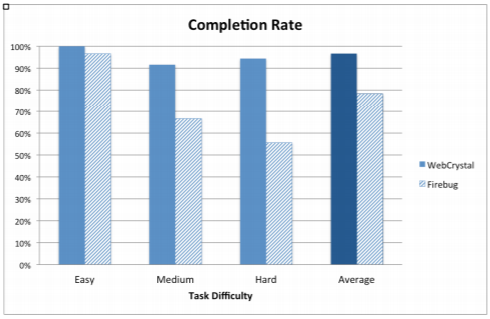
\includegraphics[width=\columnwidth]{figures/completion_rates.PNG}
    \caption{more people finished the tasks when they used our tool}  
    \label{fig:xray_screenshot}
\end{figure}

\begin{figure}
    \centering
    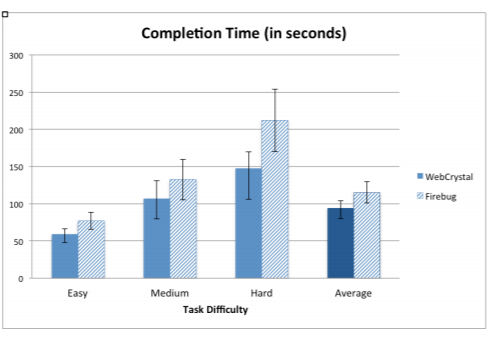
\includegraphics[width=\columnwidth]{figures/completion_time.PNG}
    \caption{people were faster when they used our tool}  
    \label{fig:xray_screenshot}
\end{figure}

\begin{figure}
    \centering
    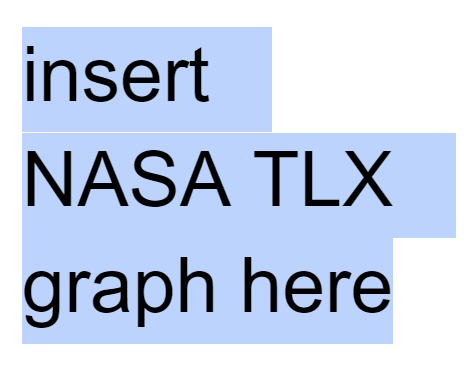
\includegraphics[width=\columnwidth]{figures/nasa_tlx.PNG}
    \caption{it was cognitively lighter to finish with the XRAY tool}  
    \label{fig:xray_screenshot}
\end{figure}

\section{Conclusion/discussion}
Discuss benefits...
\begin{itemize}
    \item promotes use of design system
    \item improves designer-developer communication
    \item this gets designers into the same medium that developers are using (ie, ``writing code'' except they are still in their comfort zone'')
    \item keeps the designers in their element: they can ignore the code entirely
    \item lets the developers get back in their element: designers are giving them code to implement instead of vague directions 

\end{itemize}

Discuss harm/risks/dangers/drawbacks...
\begin{itemize}
    \item ...I need to think about this...
\end{itemize}

Discuss limitations of our work 
\begin{itemize}
    \item margin/padding issue is not yet solved
    \item there needs to be more conversation about design systems
    \item does not support absolute positioning (cannot grab a piece of the page and move it to a different part of the web page)
    \item we didn't actually implement, but COULD implement some kind of live/real-time collaborative editing thing
    \item talk about whether or not we are really facilitating experimentation

\end{itemize}

Discuss future work/room to grow...
\begin{itemize}
    \item see the limitations and drawback sections above. 
\end{itemize}


% BALANCE COLUMNS
\balance{}

% REFERENCES FORMAT
% References must be the same font size as other body text.
% \nocite{*}
\bibliographystyle{SIGCHI-Reference-Format}
\bibliography{xray}

\end{document}

